\documentclass[journal,12pt,twocolumn]{IEEEtran}
\usepackage[top = 1in,bottom = 1in,left = 1in,right = 1in]{geometry}
\setlength{\columnsep}{2cm}
\usepackage{setspace}
\usepackage{gensymb}
\usepackage{caption}
%\usepackage{multirow}
%\usepackage{multicolumn}
%\usepackage{subcaption}
%\doublespacing
\singlespacing
\usepackage{csvsimple}
\usepackage{amsmath}
\usepackage{multicol}
%\usepackage{enumerate}
\usepackage{amssymb}
%\usepackage{graphicx}
\usepackage{newfloat}
%\usepackage{syntax}
\usepackage{listings}
\usepackage{color}
\usepackage{tikz}
\usetikzlibrary{shapes,arrows}
%\usepackage{graphicx}
%\usepackage{amssymb}
%\usepackage{relsize}
%\usepackage[cmex10]{amsmath}
%\usepackage{mathtools}
%\usepackage{amsthm}
%\interdisplaylinepenalty=2500
%\savesymbol{iint}
%\usepackage{txfonts}
%\restoresymbol{TXF}{iint}
%\usepackage{wasysym}
\usepackage{amsthm}
\usepackage{mathrsfs}
\usepackage{txfonts}
\usepackage{stfloats}
\usepackage{cite}
\usepackage{cases}
\usepackage{mathtools}
\usepackage{caption}
\usepackage{enumerate}	
\usepackage{enumitem}
\usepackage{amsmath}
%\usepackage{xtab}
\usepackage{longtable}
\usepackage{multirow}
%\usepackage{algorithm}
%\usepackage{algpseudocode}
\usepackage{enumitem}
\usepackage{mathtools}
\usepackage{hyperref}
%\usepackage[framemethod=tikz]{mdframed}
\usepackage{listings}
    %\usepackage[latin1]{inputenc}                                 %%
    \usepackage{color}                                            %%
    \usepackage{array}                                            %%
    \usepackage{longtable}                                        %%
    \usepackage{calc}                                             %%
    \usepackage{multirow}                                         %%
    \usepackage{hhline}                                           %%
    \usepackage{ifthen}                                           %%
  %optionally (for landscape tables embedded in another document): %%
    \usepackage{lscape} 
\def\inputGnumericTable{}                                 %%
\lstset{
%language=C,
frame=single, 
breaklines=true,
columns=fullflexible
}
 
\usepackage{bm}
\usepackage{caption}
\usepackage{float}
%has mini page
%to fix position (H)

\setlength{\parindent}{0pt}
%no indentation for paragraphs
\title{AI1110 ASSIGNMENT-1}
\author{Bandaru Naresh Kumar,AI21BTECH11006}
\date{}

\begin{document}

\tikzstyle{block} = [rectangle, draw,
    text width=3em, text centered, minimum height=3em]
\tikzstyle{sum} = [draw, circle, node distance=3cm]
\tikzstyle{input} = [coordinate]
\tikzstyle{output} = [coordinate]
\tikzstyle{pinstyle} = [pin edge={to-,thin,black}]

\maketitle
\section*{Exercise 1}
\subsection*{1.1}
The sample generated is
\begin{lstlisting}
https://github.com/NareshBandaru13/ASSIGNMENT1/tree/main/example%201/1.1
\end{lstlisting}
\subsection*{1.2}
The python code is
\begin{lstlisting}
https://github.com/NareshBandaru13/ASSIGNMENT1/tree/main/example%201/1.2
\end{lstlisting}
\begin{figure}[H]
    \centering
    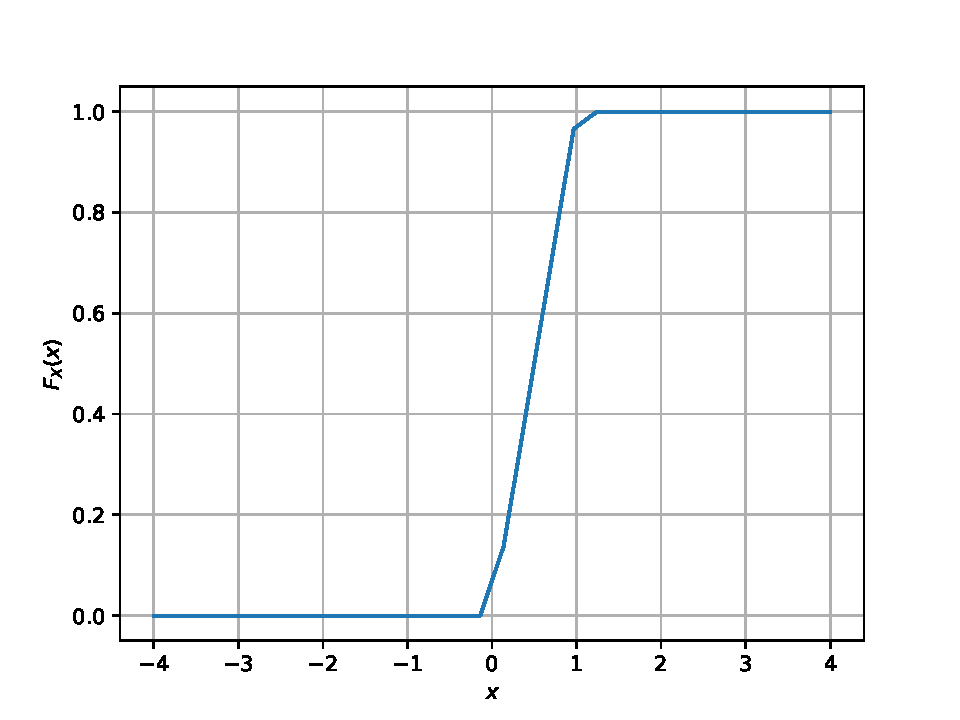
\includegraphics[scale=0.5]{figures/uni_cdf.pdf} 
    \caption{uni-cdf}
    \label{fig:my_label1}
\end{figure}
\subsection*{1.3}
Given that,\\
 U is uniform random variable.\\
So,\\
\[
  f_X (x) =
 \begin{cases}
 1  & 0 \le x \le 1 \\
 0  & otherwise \\
 \end{cases}
\]
\begin{align*}
    F_X (x) &= \int_{-\infty} ^{x} f_X (x) dx \\
          &= 0 + \int_{0} ^{x} 1 dx \\
          &= 
\begin{cases}
 1 & x >1 \\
 x & 0 \le x \le 1 \\
 0  & x<0 \\
 \end{cases}
\end{align*}

\subsection*{1.4}
The c code to find mean and variance is
\begin{lstlisting}
https://github.com/NareshBandaru13/ASSIGNMENT1/tree/main/example%201/1.4
\end{lstlisting}
\subsection*{1.5}
Given
$$E[U^{k}] = \int_{-\infty} ^{\infty} x^{k}dF_X (x)$$
\begin{enumerate}
    \item k=1 
     \begin{align*}
        E[U] &= \int_{-\infty} ^{\infty} x^{k}f_X (x) dx \\
           &= \int_{0} ^{1} x \times 1 dx \\
           &= \left[\frac{x^2}{2}\right]_{0} ^{1} = \frac{1}{2}
     \end{align*} 
     \item k=2 
       \begin{align*}
          E[U^2] &= \int_{0} ^{1} x^{2}\times 1 dx \\
          &= \left[\frac{x^3}{3}\right]_{0} ^{1} = \frac{1}{3}
      \end{align*}\\
      \begin{align*}
    variance &= E[u-E[u]]^{2} \\
    &= E[U^{2}]-E^{2}[U] \\
    &= \frac{1}{3} - \frac{1}{4} = 0.0833 \\
\end{align*}
\end{enumerate}

\section*{Exercise 2}

\subsection*{2.1}
The gau.dat file is given by
\begin{lstlisting}
https://github.com/NareshBandaru13/ASSIGNMENT1/tree/main/example%202/2.1
\end{lstlisting}

\subsection*{2.2}
cdf plot of gau.dat
\begin{lstlisting}
https://github.com/NareshBandaru13/ASSIGNMENT1/tree/main/example%202/2.2
\end{lstlisting}
\begin{figure}[H]
    \centering
    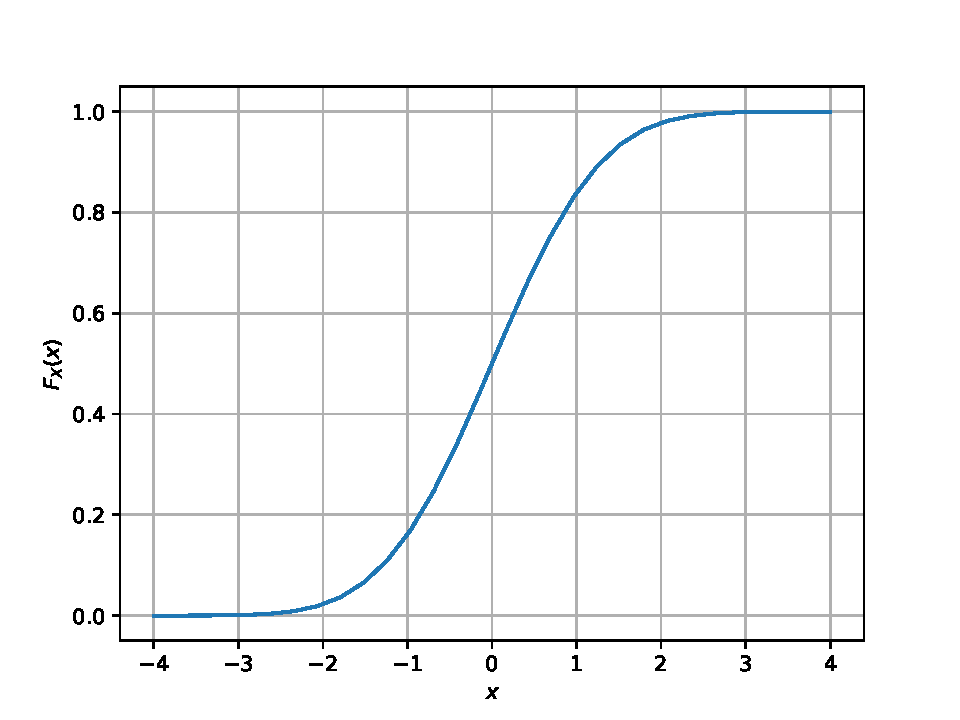
\includegraphics[scale=0.5]{figures/gauss_cdf.pdf} 
    \caption{gauss-cdf}
    \label{fig:my_cdfgau}
\end{figure}

\subsection*{2.3}
PDF of $X$ is given by
\begin{lstlisting}
https://github.com/NareshBandaru13/ASSIGNMENT1/tree/main/example%202/2.3
\end{lstlisting}
\begin{figure}[H]
    \centering
    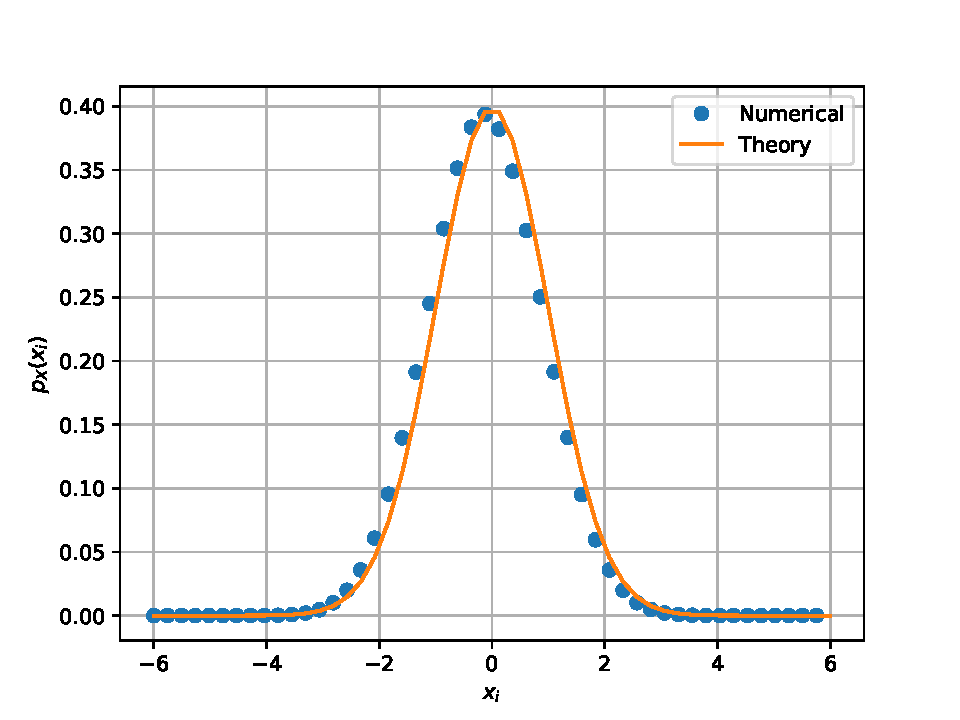
\includegraphics[scale=0.5]{figures/gauss_pdf.pdf}  
    \caption{gauss-pdf}
    \label{fig:my_label2}
\end{figure}


\subsection*{2.4}
C code to find the mean and variance
\begin{lstlisting}
https://github.com/NareshBandaru13/ASSIGNMENT1/tree/main/example%202/2.4
\end{lstlisting}

\subsection*{2.5}
Given that,
$$p_X (x) = \frac{1}{\sqrt{2\pi}}e^{-\frac{x^2}{2}} ,-\infty <x< \infty$$
By property of probability: $$\int_{-\infty} ^{\infty} p_X (x)dx = 1$$
\begin{align*}
    F_X (x) &= \int_{-\infty} ^{x} p_X (x) dx\\
     &=  \int_{-\infty} ^{x} \frac{1}{\sqrt{2\pi}}e^{-\frac{x^2}{2}} \\
     &= G(x-\mu/\sigma) \;\text{where} \mu = 0, \sigma = 1 \\
     &= G(x)
\end{align*}
Here the random variable $X\sim N(0,1)$\\
Comparing the random variable in $2.1$ :\\
$$X_0 = \sum_{i=1} ^{12} U_i -6$$
$U_i$ are independent.\\
We get:\\
$\mu _{0} = 0.0002$\\
$\sigma _{0} = 0.666$\\
As i increases, we approach normal distribution.


\section*{Exercise 3}
\subsection*{3.1}
Generated samples of $V$ and its cdf is given by
\begin{lstlisting}
https://github.com/NareshBandaru13/ASSIGNMENT1/tree/main/example%203/3.1
\end{lstlisting}
\begin{figure}[H]
    \centering
    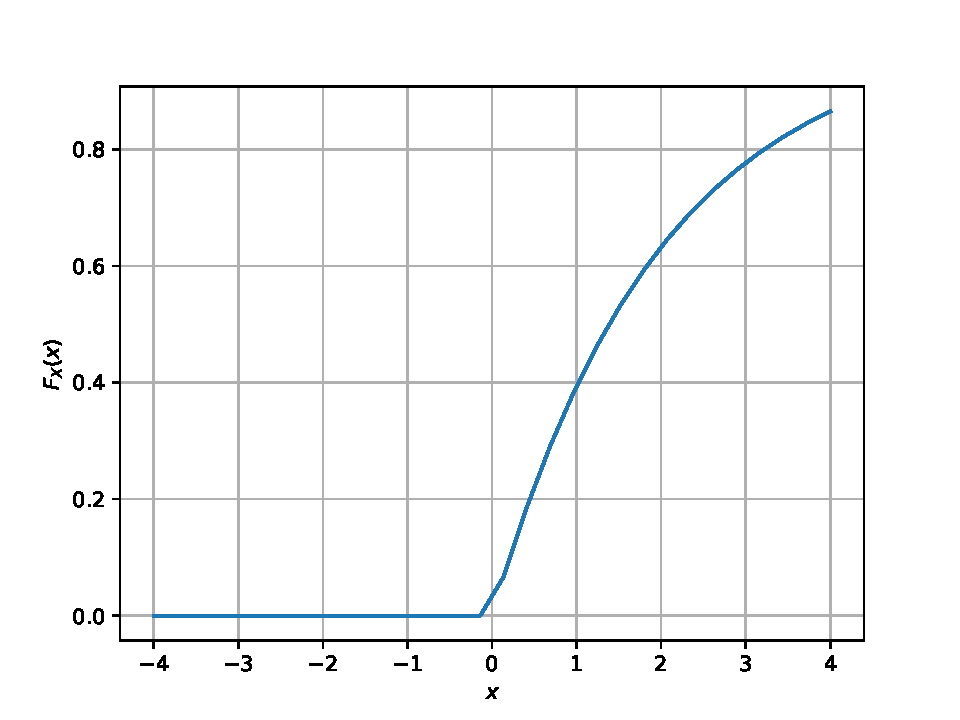
\includegraphics[scale=0.5]{figures/V_cdf.pdf}  
    \caption{V-cdf}
    \label{fig:my_label3}
\end{figure}



\subsection*{3.2}
\begin{align*}
    F_V (x) &= P\{V \le x\} \\
            &= P\{-2\times \ln{(1-U)} \le x\} \\
            &= P\{U \le 1 - e^{(-\frac{x}{2})}\} \\ 
            &= F_U\{1- e^{(-\frac{x}{2})} \}\\
            &=
\begin{cases}
 1 - e^{(-\frac{x}{2})} & 0 \le x < \infty \\
 0  & x<0 \\
 \end{cases}
\end{align*} 
\end{document}